\chapter{Research Methodology}
\label{ch:research-methodology}
\todo{Revise this entire chapter for tense issues: JG - \texttt{I did wonder about TENSE in Ch 3 – I didn’t change but to think about – all this work is DONE so use either past (my pref) or present. Not “we propose to use…” etc etc all throughout.  Especially for a by-papers thesis.  Could revised to “we proposed to use …” but I would suggest “We used …” (my pref - past) or “We use…” (present).}}

\graphicspath{{mainmatter/research-methodology/figures/}}

\label{sec:research-methodology:preface}

Investigating software engineering practices is often a complex task as it is imperative to understand the social and cognitive processes around software engineers and not just the tools and processes used \citep{Easterbrook:2007ws}. This chapter explores our research methodology by exploring five key elements of empirical software engineering research: firstly, (i) we provide an extended focus to the study by reviewing our research questions (see \cref{sec:introduction:goals}) anchored under the context of an existing research question classification taxonomy, (ii) characterise our research goals through an explicit philosophical stance, (iii) explain how the stance selected impacts our selection of research methods and data collection techniques (by dissecting our choice of methods used to reach these research goals), (iv) discuss a set of criteria for assessing the validity of our study design and the findings of our research, and lastly (v) discuss the practical considerations of our chosen methods. 

The foundations for developing this research methodology has been expanded from that proposed by \citet{Easterbrook:2007ws}, \citet{Wohlin:2014jq}, \citet{Wohlin:2012bu} and \citet{Shaw:2003aa}.

\section{Research Questions Revisited}
\label{sec:research-methodology:research-questions}

%In \cref{sec:introduction:goals}, we rq:nature:runtime to three hypotheses: (i) \glspl{cvs} have non-deterministic properties that confuse developers with a deterministic mindset; (ii) the implicit risks to using these services without fully appreciating their unintended side effects has an impact to software quality; (iii) the service providers do not sufficiently document these behavioural and evolution issues.

To discuss our research strategy, we revisit our \NumPrimaryRQs{} primary and \NumSecondaryRQs{} secondary research questions (RQs) through the classification technique discussed by \citet{Easterbrook:2007ws}, a technique originally proposed in the field of psychology by \citet{Meltzoff:1998wg} but adapted to software engineering. A summary of the classifications made to our research questions are presented in \cref{tab:research-methodology:rqs}.

Our research study involves a mix of \NumEmpiricalRQs{} \textit{empirical}\footnote{Or `knowledge' questions, that extend our \textit{knowledge} on certain phenomena.} RQs, that focus on observing and analysing existing phenomena, and \NumNonEmpiricalRQs{} \textit{non-empirical} RQs, that focuses on designing better approaches to solve software engineering tasks \citep{Simon:1996uw}. The use of empirical \textit{and} non-empirical RQs are best combined in long-term software engineering research studies where the phenomena are under-explored, as is the case with \glspl{cvs}. Further, these approaches help propose solutions to issues found in the phenomena studied \citep{Wieringa:2006vd}. We discuss both our empirical and non-empirical RQs in \cref{ssec:research-methodology:research-questions:empirical,ssec:research-methodology:research-questions:nonempirical} below. 

\begin{table}[tbh]
\centering
\caption[Classification of research questions in this thesis]{A summary of our research questions classified using the strategies presented by \citet{Easterbrook:2007ws} and \citet{Meltzoff:1998wg}.}\label{tab:research-methodology:rqs}
\tablefit{\begin{tabular}{p{0.07\linewidth}p{0.55\linewidth}|p{0.13\linewidth}p{.33\linewidth}}
\toprule
\textbf{\#}&
\textbf{RQ}&
\textbf{Primary/ Secondary}&
\textbf{RQ Classification}
\\
\midrule
\midrule
\ref{rq:nature} &
\RQOneTextLandscapeAnalysis{} &
Primary &
\makecell[tl]{
\textsc{Empirical}\\
$\hookrightarrow$~\textit{Exploratory}\\
$~~\hookrightarrow$~\textit{Description/Classification}
}
\\
\ref{rq:nature:runtime} &
\RQOneTextLandscapeAnalysisRuntime{} &
Secondary &
\makecell[tl]{
\textsc{Empirical}\\
$\hookrightarrow$~\textit{Exploratory}\\
$~~\hookrightarrow$~\textit{Description/Classification}
}
\\
\ref{rq:nature:evolution} &
\RQOneTextLandscapeAnalysisEvolution{} &
Secondary &
\makecell[tl]{
\textsc{Empirical}\\
$\hookrightarrow$~\textit{Exploratory}\\
$~~\hookrightarrow$~\textit{Description/Classification}
}
\\
\midrule
\ref{rq:docs} &
\RQTwoTextDocumentation{}&
Primary &
\makecell[tl]{
\textsc{Empirical}\\
$\hookrightarrow$~\textit{Exploratory}\\
$~~\hookrightarrow$~\textit{Existence}
}
\\
\ref{rq:docs:complete} &
\RQTwoTextDocumentationWhatIsCompleteDocs{}&
Secondary &
\makecell[tl]{
\textsc{Empirical}\\
$\hookrightarrow$~\textit{Exploratory}\\
$~~\hookrightarrow$~\textit{Composition}
}
\\
\ref{rq:docs:missing} &
\RQTwoTextDocumentationMissingAttributes{}&
Secondary &
\makecell[tl]{
\textsc{Non-Empirical}\\
$\hookrightarrow$~\textit{Design}\\
}
\\
\midrule
\ref{rq:devs} &
\RQThreeTextDevMiscomprehension{}&
Primary &
\makecell[tl]{
\textsc{Empirical}\\
$\hookrightarrow$~\textit{Exploratory}\\
$~~\hookrightarrow$~\textit{Descriptive-Comparative}
}
\\
\ref{rq:devs:issues} &
\RQThreeTextDevMiscomprehensionIssueTypes{}&
Secondary &
\makecell[tl]{
\textsc{Empirical}\\
$\hookrightarrow$~\textit{Base-Rate}\\
$~~\hookrightarrow$~\textit{Frequency/Distribution}
}
\\
\ref{rq:devs:frustration} &
\RQThreeTextDevMiscomprehensionFrustration{} &
Secondary &
\makecell[tl]{
\textsc{Empirical}\\
$\hookrightarrow$~\textit{Exploratory}\\
$~~\hookrightarrow$~\textit{Description/Classification}
}
\\
\ref{rq:devs:vs-traditional} &
\RQThreeTextDevMiscomprehensionVsConventional{} &
Secondary &
\makecell[tl]{
\textsc{Empirical}\\
$\hookrightarrow$~\textit{Base-Rate}\\
$~~\hookrightarrow$~\textit{Frequency/Distribution}
}
\\
\midrule
\ref{rq:design} &
\RQFourDesign{} &
Primary &
\makecell[tl]{
\textsc{Non-Empirical}\\
$\hookrightarrow$~\textit{Design}\\
}
\\
\bottomrule
\end{tabular}}
\end{table}


\subsection{Empirical Research Questions}
\label{ssec:research-methodology:research-questions:empirical}

In total, \NumEmpiricalRQs{} empirically-based RQs are posed in this study to help us understand the way developers currently interact and work with web services that provide computer vision. The majority of these questions are \textit{exploratory} questions that contribute to a landscape analysis of these services (\ref{rq:nature}, \ref{rq:nature:runtime} and \ref{rq:nature:evolution}), how well they are documented (\ref{rq:docs}), and the issues developers currently face when using them (\ref{rq:devs}). Our other exploratory questions complement the answers to these questions. For instance, to understand if \glspl{cvs} are sufficiently documented (an \textit{existence} exploratory question posed in \ref{rq:docs}), we need to understand the components of a `sufficient' or `complete' \gls{api} document via \ref{rq:docs:complete} as proposed in both the literature and by software developers. While \ref{rq:docs:complete} does not directly relate to \glspl{cvs}, answering it gives us an understanding the components of complete \gls{api} documentation, and therefore, we can assess what aspects they are missing and where improvements can be made (\ref{rq:docs:missing}). These questions are \textit{descriptive and classification} questions that help describe and classify what practices are in use for existing \gls{cvs} \gls{api} documentation and the nature behind these services. Answering these exploratory questions assists in refining preciser terms of the phenomena, ways in which we find evidence for them and ensuring the data found is valid.

By answering these questions, we have a clearer understanding of the phenomena; we then follow up by posing \NumBaseRateRQs{} additional \textit{base-rate questions} that helps provide a basis to confirm that the phenomena occurring is normal (or unusual) behaviour by investigating the patterns of phenomena's occurrence against other phenomena. \ref{rq:devs:issues} is a \textit{frequency and distribution} question to help us understand what types of issues developers often encounter most, given a lack of formal extended training in artificial intelligence. This achieves us an insight into the developer's mindset and regular thought patterns toward these \glspl{api}. We can then contrast this distribution using our second base-rate question (\ref{rq:devs:vs-traditional}), that assesses the distributional differences between these intelligent components and non-intelligent (conventional) software components. Combined, these two questions can help us answer how the issues raised against \glspl{cvs} are different to normal \glslong{so} issues---our \textit{descriptive-comparative} question posed in \ref{rq:devs}---and, similarly, we can classify and rank which issues developers find most frustrating (\ref{rq:devs:frustration}).

%Lastly, we investigate the relationship between the improved documentation and improvements to other aspects of the software development process. Chiefly, \ref{rqs:implications:do-metrics-improve} is concerned with whether any improvements to metadata or documentation correlate to improvements in software quality, developer productivity, or developer education (and is a \textit{relationship establishment question}). If we establish such a relationship, we refine the question and investigate the specific causes using three \textit{causality questions} defined under \ref{rqs:implications:aspects}, namely by associating three classes of measurable metrics (internal quality metrics, external quality metrics, developer education insight metrics) to the improved documentation.

\subsection{Non-Empirical Research Questions}
\label{ssec:research-methodology:research-questions:nonempirical}

\ref{rq:docs:missing} and \ref{rq:design} are both non-empirically-based \textit{design questions}; they are concerned with ways in which we can improve a \gls{cvs} by investigating what additional attributes are needed in both the documentation of \glspl{cvs} and in the integration architectures developers can employ to improve reliability and robustness in their applications. They are not classified as empirical questions as we investigate what \textit{will be} and not \textit{what is}. By understanding the process by which developers desire additional attributes of documentation and integration strategies, we can help shape improvements to the existing designs of using \glspl{cvs}.
\section{Philosophical Stances}
\label{sec:research-methodology:philosophical-stances}

Philosophical stances guide the researcher's action by fortifying what constitutes `valid truth' against a fundamental set of core beliefs \citep{Ritzer:1991ge}. In software engineering, four dominant philosophical stances are commonly characterised \citep{Creswell:2017vn,Petersen:2019ji}: positivism (or post-positivism), constructivism (or interpretivism), pragmatism, and critical theory (or advocacy/participatory). To construct such a `validity of truth', we will review these four philosophical stances in this section, and state the stance that we explicitly adopt and our reasoning for this.

\subsubsection{Positivism}
Positivists claim truth to be all observable facts, reduced piece-by-piece to smaller components which is incrementally verifiable to form truth. We do not base our work on the positivistic stance as the theories governing verifiable hypothesis must be precise from the start of the research. Moreover, due to its reductionist approach, it is difficult to isolate these hypotheses and study them in isolation from context.
As our hypotheses are not context-agnostic, we steer clear from this stance.

\subsubsection{Constructivism}
Constructivists see knowledge embedded within the human context; truth is the \textit{interpretive} observation by understanding the differences in human thought between meaning and action \citep{Klein:1999uv}. That is, the interpretation of the theory is just as important to the empirical observation itself.
We partially adopt a constructivist stance as we attempt to model the developer's mindset, being an approach that is rich in qualitative data on human activity.

\subsubsection{Pragmistism}
Pragmatism is a less dogmatic approach that encourages the incomplete and approximate nature of knowledge and is dependent on the methods in which the knowledge was extracted. The utility of consensually agreed knowledge is the key outcome, and is therefore relative to those who seek utility in the knowledge---what is the useful for one person is not so for the other. While we value the utility of knowledge, it is difficult to obtain consensus especially on an ill-researched topic such as ours, and therefore we do not adopt this stance.

\subsubsection{Critical Theory}
This study chiefly adopts the philosophy of critical theory \citep{Calhoun:1995ww}. A key outcome of the study is to shift the developer's restrictive deterministic mindset and shed light on developing a new framework actively with the developer community that seeks to improve the process of using such \glspl{api}. In software engineering, critical theory is used to ``actively [seek] to challenge existing perceptions about software practice'' \citep{Easterbrook:2007ws}, and this study utilises such an approach to shift the mindset of \gls{cvs} consumers and providers alike on how the documentation and metadata should not be written with the `traditional' deterministic mindset at heart. Thus, our key philosophical approach is critical theory to seek out \textit{what-can-be} using  partial constructivism to model the current \textit{what-is}.

\section{Research Methods}
\label{sec:research-methodology:review}

Research methods are ``a set of organising principles around which empirical data is collection and analysed'' \citep{Easterbrook:2007ws}. \citet{Creswell:2017vn} suggests that strong research design is reflected when the weaknesses of multiple methods complement each other. Using a mixed-methods approach is therefore commonplace in software engineering research, typically due to the human-oriented nature investigating how software engineers work both individually (where methods from psychology may be employed) and together (where methods from sociology may be employed).

Therefore, studies in software engineering are typically performed as field studies where researchers and developers (or the artefacts they produce) are analysed either directly or indirectly \citep{Singer:2007tu}. The mixed-methods approach combines five classes of field study methods (or empirical strategies/studies) most relevant in empirical software engineering research \citep{Easterbrook:2007ws, Wohlin:2012bu, Juristo:2013vj}: controlled experiments, case studies, survey research, ethnographies, and action research. We chiefly adopt a mixed-methods approach to our work using the \textit{concurrent triangulation} mixed-methods strategy \citep{Jick:1979el} as it best compensates for weaknesses that exist in all research methods, and employs the best strengths of others \citep{Creswell:2017vn}.

\subsection{Review of Relevant Research Methods}
\label{ssec:research-methodology:review:methods}

Below we review some of the research methods most relevant to our research questions as refined in \cref{sec:research-methodology:research-questions} as presented by \citet{Easterbrook:2007ws}.

\subsubsection{Controlled Experiments}
A controlled experiment is an investigation of a clear, testable hypothesis that guides the researcher to decide and precisely measure how at least one independent variable can be manipulated and effect at least one other dependent variable. They determine if the two variables are related and if a cause-effect relationship exists between them. The combination of independent variable values is a \textit{treatment}. It is common to recruit human subjects to perform a task and measure the effect of a randomly assigned treatment on the subjects, though it is not always possible to achieve full randomisation in real-life software engineering contexts, in which case a \textit{quasi-experiment} may be employed where subjects are not randomly assigned to treatments.

While we have well-defined RQs, refining them into precise, \textit{measurable} variables is challenging due to the qualitative nature they present. A well-defined population is also critical and must be easily accessible; the varied range of beginner to expert software engineers with varied understanding of artificial intelligence concepts is required to perform controlled experiments, and thus recruitment may prove challenging. Lastly, the controlled experiment is essentially reductionist by affecting a small amount of variables of interest and controlling all others. This approach is too clinical for the practical outcomes by which our research goals aim for, and is therefore closely tied to the positivist stance.

\subsubsection{Case Studies}
Case studies investigate phenomena in their real-life context and are well-suited when the boundary between context and phenomena is unknown \citep{Yin:2017tf}. They offer understanding of how and why certain phenomena occur, thereby investigating ways cause-effect relationships can occur. They can be used to test existing theories (\textit{confirmatory case studies}) by refuting theories in real-world contexts instead of under laboratory conditions or to generate new hypotheses and build theories during the initial investigation of some phenomena (\textit{exploratory case studies}).

Case studies are well-suited where the context of a situation plays a role in the phenomenon being studied. They also lend themselves to purposive sampling rather than random sampling, and thus it is possible to selectively choose cases that benefit our research goals and (using our critical theorist stance) select cases that will actively benefit our participant software engineering audience most to draw attention to situations regarded as problematic in \gls{cvs}.

\subsubsection{Survey Research}
Survey research identifies characteristics of a broad population of individuals through direct data collection techniques such as interviews and questionnaires or independent techniques such as data logging. Defining that well-defined population is critical, and selecting a representative sample from it to generalise the data gathered usually assists in answering base-rate questions.

By identifying representative sample of the population, from beginner to experienced developers with varying understanding of \gls{cvs} \glspl{api}, we can use survey research to assist in answering our exploratory and base-rate RQs (see \cref{ssec:research-methodology:research-questions:empirical}) in determining the qualitative aspects of how individual developers perceive and work with the existing \glspl{api}, either by directly asking them, or by mining third-party discussion websites such as \glsx{so}. Similarlly, we can use this strategy to assess the developer's understanding on what makes \gls{api} documentation sufficient by assessing whether specific factors suggested from literature are useful according to developers. However, with direct survey research techniques, low response rates may prove challenging, especially if no inducements can be offered for participation.

\subsubsection{Ethnographies}
Ethnographies investigates the understanding of social interaction within community through field observation \citep{Robinson:2007tp}. Resulting ethnographies help understand how software engineering technical communities build practices, communication strategies and perform technical work collaboratively.

Ethnographies require the researcher to be highly trained in observational and qualitative data analysis, especially if the form of ethnography is participant observation, whereby the researcher is embedded of the technical community for observation. This may require the longevity of the study to be far greater than a couple of weeks, and the researcher must remain part of the project for its duration to develop enough local theories about how the community functions. While it assists in revealing subtle but important aspects of work practices within software teams, this study does not focus on the study of teams, and is therefore not a research method relevant to this project.


\subsubsection{Action Research}
Action researchers simultaneously solve real-world problems while studying the experience of solving the problem \citep{Davison:2004wo} by actively seeking to intervene in the situation for the purpose of improving it. A precondition is to engage with a \textit{problem owner} who is willing to collaborate in identifying and solving the problem faced. The problem must be authentic (a problem worth solving) and must have new knowledge outcomes for those involved. It is also characterised as an iterative approach to problem solving, where the knowledge gained from solving the problem has a desirable solution that empowers the problem owner and researcher.

This research is most associated to our adopted philosophical stance of critical theory. As this project is being conducted under the \gls{a2i2} collaboratively with engaged industry clients, we have identified a need for solving an authentic problem that industry faces. The desired outcome of this project is to facilitate wider change in the usage and development of \glspl{cvs}; thus, engaging action research as a potential method throughout the mixed-methods approach is used in this research.

\subsection{Review of Data Collection Techniques for Field Studies}
\label{ssec:research-methodology:review:techniques}

\citeauthor{Singer:2007tu} developed a taxonomy \citep{Singer:2007tu,Lethbridge:2005jv} showcasing data collection techniques in field studies that are used in conjunction with a variety of methods based on the level of interaction between researcher and software engineer, if any. This taxonomy is reproduced in \cref{fig:research-methodology:review:field-techniques}, where techniques used in this research study are starred.

\afterpage{\begin{landscape}
\begin{table}
\centering
\caption[Review of field study techniques]{Questions asked by software engineering researchers (column 2) that can be answered by field study techniques. (Adapted from \citep{Singer:2007tu}.) Methods used within this research study are starred.}
\label{fig:research-methodology:review:field-techniques}
\tablefitlandscape{1.05}{
\begin{tabular}{p{0.2\linewidth}|p{0.375\linewidth}p{0.125\linewidth}p{0.3\linewidth}}
\toprule
\textbf{Technique} &
\textbf{Used by researchers when their goal is to understand...} &
\textbf{Volume of data} &
\textbf{Also used by software engineers for...}\\

\midrule
\midrule
\multicolumn{4}{l}{\textsc{\textbf{Direct Techniques}}}\\
\midrule

Brainstorming and focus groups &
Ideas and general background about the process and product, general opinions (also useful to enhance participant rapport) &
Small &
Requirements gathering, project planning \\

Interviews and questionnaires &
General information (including opinions) about process, product, personal knowledge etc. &
Small to large &
Requirements and evaluation \\

Conceptual modelling &
Mental models of product or process. &
Small &
Requirements \\

Work diaries &
Time spent or frequency of certain tasks (rough approximation, over days or weeks) &
Medium &
Time sheets \\

Think-aloud sessions &
Mental models, goals, rationale and patterns of activities &
Medium to large &
UI evaluation \\

Shadowing and observation &
Time spent or frequency of tasks (intermittent over relatively short periods), patterns of activities, some goals and rationale &
Small &
Advanced approaches to use case or task analysis \\

Participant observation (joining the team) &
Deep understanding, goals and rationale for actions, time spent or frequency over a long period &
Medium to large &
-- \\

\midrule
\multicolumn{4}{l}{\textsc{\textbf{Indirect Techniques}}}\\
\midrule

Instrumenting systems &
Software usage over a long period, for many participants &
Large &
Software usage analysis \\

Fly on the wall &
Time spent intermittently in one location, patterns of activities (particularly collaboration) &
Medium &
-- \\

\midrule
\multicolumn{4}{l}{\textsc{\textbf{Independent Techniques}}}\\
\midrule

Analysis of work databases &
Long-term patterns relating to software evolution, faults etc. &
Large &
Metrics gathering \\

Analysis of tool use logs &
Details of tool usage &
Large &
-- \\

Documentation analysis &
Design and documentation practices, general understanding &
Medium &
Reverse engineering \\

Static and dynamic analysis &
Design and programming practices, general understanding &
Large &
Program comprehension, metrics, testing, etc. \\

\bottomrule

\end{tabular}}
\end{table}\end{landscape}}
\section{Research Design}
\label{sec:research-methodology:review}

Research methods are ``a set of organising principles around which empirical data is collection and analysed'' \citep{Easterbrook:2007ws}. \citet{Creswell:2017vn} suggests that strong research design is reflected when the weaknesses of multiple methods complement each other. Using a mixed-methods approach is therefore commonplace in software engineering research, typically due to the human-oriented nature investigating how software engineers work both individually (where methods from psychology may be employed) and together (where methods from sociology may be employed). 

Therefore, studies in software engineering are typically performed as field studies where researchers and developers (or the artefacts they produce) are analysed either directly or indirectly \citep{Singer:2007tu}. The mixed-methods approach combines five classes of field study methods (or empirical strategies/studies) most relevant in empirical software engineering research \citep{Easterbrook:2007ws, Wohlin:2012bu, Juristo:2013vj}: controlled experiments, case studies, survey research, ethnographies, and action research. We chiefly adopt a mixed-methods approach to our work using the \textit{concurrent triangulation} mixed-methods strategy \citep{Jick:1979el} as it best compensates for weaknesses that exist in all research methods, and employs the best strengths of others.



\subsection{Review of Relevant Research Methods}
\label{ssec:research-methodology:review:methods}

Below we review some of the research methods most relevant to our research questions as refined in \cref{sec:research-methodology:research-questions} as presented by \citet{Easterbrook:2007ws}.

\paragraph{Controlled Experiments}
A controlled experiment is an investigation of a clear, testable hypothesis that guides the researcher to decide and precisely measure how at least one independent variable can be manipulated and effect at least one other dependent variable. They determine if the two variables are related and if a cause-effect relationship exists between them. The combination of independent variable values is a \textit{treatment}. It is common to recruit human subjects to perform a task and measure the effect of a randomly assigned treatment on the subjects, though it is not always possible to achieve full randomisation in real-life software engineering contexts, in which case a \textit{quasi-experiment} may be employed where subjects are not randomly assigned to treatments.

While we have defined hypotheses (\rh{1}--\rh{3}), refining them into precise, measurable variables is challenging due to the qualitative nature they present. A well-defined population is also critical and must be easily accessible; the varied range of beginner to expert software engineers with varied understanding of artificial intelligence concepts is required to perform controlled experiments, and thus recruitment may prove challenging. Lastly, the controlled experiment is essentially reductionist by affecting a small amount of variables of interest and controlling all others. This approach is too clinical for the practical outcomes by which our research goals aim for, and is therefore closely tied to the positivist stance.

\paragraph{Case Studies}
Case studies investigate phenomena in their real-life context and are well-suited when the boundary between context and phenomena is unknown \citep{Yin:2017tf}. They offer understanding of how and why certain phenomena occur, thereby investigating ways cause-effect relationships can occur. They can be used to test existing theories (\textit{confirmatory case studies}) by refuting theories in real-world contexts instead of under laboratory conditions or to generate new hypotheses and build theories during the initial investigation of some phenomena (\textit{exploratory case studies}).

Case studies are well-suited where the context of a situation plays a role in the phenomenon being studied, which we specifically relate back to \rh{2} (\ref{rqs:metadata:what-problems-du                                                                e-to-lack-of-metadata} and \ref{rqs:metadata:what-metadata-do-devs-want-and-why}) in exploring whether the context of an application using an \gls{iws} requires the \gls{iws} context-specific or of context-agnostic. They also lend themselves to purposive sampling rather than random sampling, and thus we can selective choose cases that benefit the research goal of \rh{2} and (using our critical theorist stance) select cases that will actively benefit our participant software engineering audience most to draw attention to situations regarded as most problematic.

\paragraph{Survey Research}
Survey research identifies characteristics of a broad population of individuals through direct data collection techniques such as interviews and questionnaires or independent techniques such as data logging. Defining that well-defined population is critical, and selecting a representative sample from it to generalise the data gathered usually assists in answering base-rate questions.

By identifying representative sample of the population, from beginner to experienced developers with varying understanding of \gls{iws} \glspl{api}, we can use survey research to assist in answering our exploratory and base-rate research questions under \rh{1} and \rh{2} (see \cref{ssec:research-methodology:research-questions:knowledge-questions}) in determining the qualitative aspects of how individual developers perceive and work with the existing \glspl{api}, either by directly asking them or by mining third-party discussion websites such as \glsx{so}. However, with direct survey research techniques, low response rates may prove challenging, especially if no inducements can be offered for participation.

\paragraph{Ethnographies}
Ethnographies investigates the understanding of social interaction within community through field observation \citep{Robinson:2007tp}. Resulting ethnographies help understand how software engineering technical communities build practices, communication strategies and perform technical work collaboratively. 

Ethnographies require the researcher to be highly trained in observational and qualitative data analysis, especially if the form of ethnography is participant observation, whereby the researcher is embedded of the technical community for observation. This may require the longevity of the study to be far greater than a couple of weeks, and the researcher must remain part of the project for its duration to develop enough local theories about how the community functions. While it assists in revealing subtle but important aspects of work practices within software teams, this study does not focus on the study of teams, and is therefore not a research method relevant to this project.


\paragraph{Action Research}
Action researchers simultaneously solve real-world problems while studying the experience of solving the problem \citep{Davison:2004wo} by actively seeking to intervene in the situation for the purpose of improving it. A precondition is to engage with a \textit{problem owner} who is willing to collaborate in identifying and solving the problem faced. The problem must be authentic (a problem worth solving) and must have new knowledge outcomes for those involved. It is also characterised as an iterative approach to problem solving, where the knowledge gained from solving the problem has a desirable solution that empowers the problem owner and researcher. 

This research is most associated to our adopted philosophical stance of critical theory. As this project is being conducted under the \gls{a2i2} collaboratively with engaged industry clients, we have identified a need for solving an authentic problem that industry faces. The desired outcome of this project is to facilitate wider change in the usage and development of \glspl{cvs}; thus, engaging action research as a primary method throughout the mixed-methods approach used in this research.

\subsection{Review of Data Collection Techniques for Field Studies}
\label{ssec:research-methodology:review:techniques}

\citeauthor{Singer:2007tu} developed a taxonomy \citep{Singer:2007tu,Lethbridge:2005jv} showcasing data collection techniques in field studies that are used in conjunction with a variety of methods based on the level of interaction between researcher and software engineer, if any. This taxonomy is reproduced in \cref{fig:research-methodology:review:field-techniques}.

\section{Proposed Experiments}
\label{sec:research-methodology:experiments}

This section discusses two proposed experiments that we conduct in this study. For each experiment, we describe an overview of the experiment grounded known methods and techniques (\cref{ssec:research-methodology:review:methods,ssec:research-methodology:review:techniques}), our approach to analysing the data, as well as linking the experiment back to a research hypothesis and question (\cref{sec:introduction:hypohtesis}). A high-level overview of the proposed experiments and the major bodies of work they encompass is presented in \cref{fig:research-methodology:review:activity-diagram}.

\begin{figure}[t!]
  \centering
  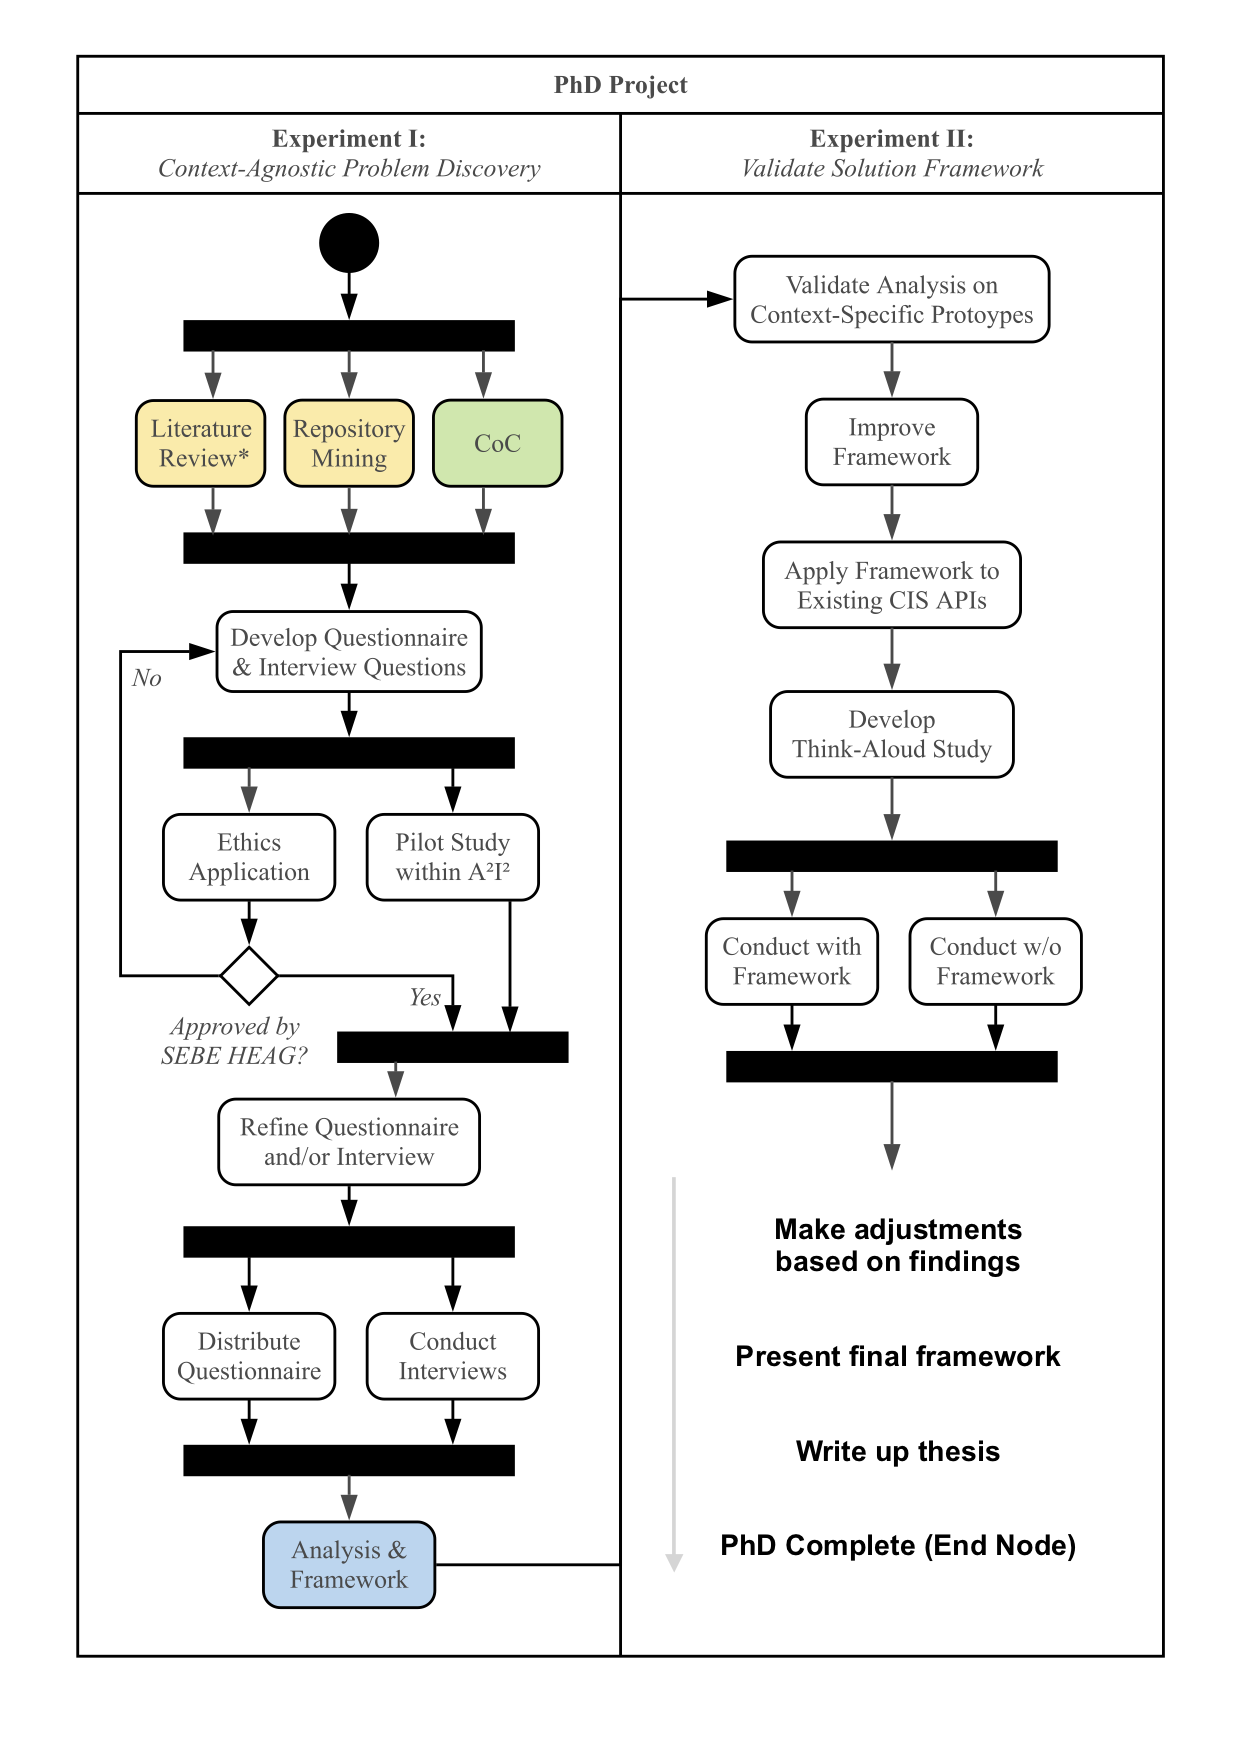
\includegraphics[width=0.9\linewidth]{experiment-activity-diagram}
  \caption[High-level overview of the proposed experiments]{High-level activity diagram of the proposed experiments in this study. Literature review is ongoing.}
  \label{fig:research-methodology:review:activity-diagram}
\end{figure}


\subsection{Experiment I: Develop Initial Framework}
\label{ssec:research-methodology:experiments:1}

Experiment I shapes a context-agnostic approach to understand current usage patterns of \gls{iws} \glspl{api} and the ways by which developers interpret them. Briefly, this experiment is comprised under two phases of field survey research: (i) repository mining developer discussion forums (i.e., analysis of databases and documentation analysis) to understand what developers currently complain about on these forums and where their mismatch in understanding lies; (ii) conducting unstructured interviews and distributing a questionnaire to gather personal opinion based on individual developer's anecdotal remarks.

\subsubsection{Relevance and Motivation}

Experiment I aims to better understand the existing mindsets that developers have when approaching to use \glsplx{cvs}. This work therefore ties in to \rh{1}; by understanding the developer mindset in how they interpret \gls{cvs} \glspl{api}, we are better informed to produce a framework that increases the effectiveness of the documentation of those existing \gls{cvs} providers.

\rh{1} postulates that the software engineering community do not fully understand the `magic' behind \gls{iws} \glspl{api}. As described in \cref{sec:introduction:hypohtesis}, they face a gap in their understanding around the underlying architecture of pre-built, machine learnt \glspl{api} (\ref{rqs:apidoc:how-do-devs-understand-it}). Software developers are not well-supported by the \gls{iws} providers, and therefore do not have a consistent set of common best practices when approaching to use these \glspl{api} (\ref{rqs:apidoc:what-is-in-use}). It is therefore necessary that \gls{iws} providers provide additional information to gap this mismatched understanding (\ref{rqs:apidoc:what-additional-information-needed}). 

\subsubsection{Data Collection \& Analysis}

\paragraph{Phase 1: Repository Mining}
Developers typically congregate in search of discourses on issues they face in online forums, such as \glsx{so} and Quora, as well as writing their experiences in personal blogs such as Medium. The simplest of these platforms is \gls{so} (a sub-community of the Stack Exchange family of targeted communities) that specifically targets developer issues on using a simple Q\&A interface, where developers can discuss technical aspects and general software development topics. Moreover, \gls{so} is often acknowledged as \textit{the} `go-to' place for developers to find high-quality code snippets that assist in their problems \citep{Subramanian:2014bg}.

Thus, to begin validating \gls{iws} \gls{api} usage and misunderstanding in a generalised context (i.e., context-agnostic to the project at hand), we propose using repository mining on \gls{so} to help answer our research questions. Specifically, we select \gls{so} due to its targeted community of developers\footnote{We also acknowledge that there are other targeted software engineering Stack Exchange communities such as Stack Exchange Software Engineering (\url{https://softwareengineering.stackexchange.com}), though (as of January 2019) this much smaller community consists of only 52,000 questions versus \gls{so}'s 17 million.} and the availability of its publicly available dataset released as `data dumps' on the Stack Exchange Data Explorer\footnoteurl{https://data.stackexchange.com/stackoverflow}{17 January 2017} and Google BigQuery\footnoteurl{https://console.cloud.google.com/marketplace/details/stack-exchange/stack-overflow}{17 January 2017}. Studies conducted have also used \gls{so} to mine developer discourse \citep{Choi:2015wo,Sinha:2013tt,Novielli:2015vda,Rosen:2016uk,Pal:2012te,Bajaj:2014wg,LinaresVasquez:2014vj,Wang:2013ue,Barua:2012gz,Reboucas:2016tw,Allamanis:2013is,Tahir:2018ks}.

Due to the enormity of the data produced, we will use qualitative analysis on the questions mined using assistive tools such as NVivo. For this, we will conduct a thematic analysis on the themes of each question mined, the relevance of the question to our research topic, and ensuring strict coding schemes (that reflect our research goals) are adhered to. We refer to \citet{Singer:2007tu} and \citet{Miles:1994ty} on coding and analysing this qualitative data gathered.

\paragraph{Phase 2: Personal Opinion Surveys}
We follow the triangulation approach proposed by \citet{Jick:1979el} to corroborate the qualitative data of developers' discussion of \gls{so} with secondary survey research, thereby validating what people say on git with what is said and done in real life. \citet{Kitchenham:2007ux} provide an introduction on methods used to conduct personal opinion surveys which we adopt as an initial reference in (i) shaping our survey objectives around our research goals, (ii) designing a cross-sectional survey, (iii) developing and evaluating our two survey instruments (consisting of a structured questionnaire and semi-structured interview), (iv) evaluating our instruments, (v) obtaining the data and (vi) analysing the data.

As is good practice in developing questionnaire instruments to evaluate their reliability and validity \citep{Litwin:1995wt}, we evaluate our instrument design by asking colleagues to critique it via pilot studies within \gls{a2i2}. This assists in identifying any problems with the questionnaire itself and with any issues that may occur with the response rate and follow-up procedures. We follow a similar approach by practicing the interview instrument on colleagues within \gls{a2i2}.

Findings from the pilot study helps inform us for a widely distributed questionnaire and conducting interviews out in the field, where we recruit external software engineers in industry through the industry contacts of \gls{a2i2}. Ethics approval from the Faculty of Science, Engineering and Built Environment Human Ethics Advisory Group (SEBE HEAG) will be required prior to externally conducting this survey research (see \cref{ch:ethics}). The quantitative (survey) and qualitative (interview) analysis allows us to shape the research outcome of \rh{1}---an \gls{api} documentation quality assessment framework---and assists in stabilising our general understanding of how developers use these existing \glspl{api}.

\subsection{Developing the Initial Framework}

Our initial framework is developed using the qualitative and quantitative analyses from the findings of Experiment I. As this is a creative phase in which we are developing a new framework, the exact process by which we develop the initial framework will come to light once more insight is determined. However it is anticipated discussion with other researchers and engineers at \gls{a2i2} about the analyses of the findings (i.e., white-boarding sessions of potential ideas from the findings) will help develop our initial documentation framework. This framework will take the shape of a checklist or table, typical of information systems studies (e.g., \citep{Lau:1999vs}), that indicate what attributes should be best suited for what needs.

\subsection{Experiment II: Validate Initial Framework}
\label{ssec:research-methodology:experiments:2}

Experiment II extends the \textit{generalised} context of Experiment I by evaluating how the findings of Experiment I translates to context-specific applications. We confirm that the generalised findings are (indeed) genuine by conducting action research in combination with an observational study on software engineers. This experiment is also compromised of: (i) development of prototypes using \gls{iws} \glspl{api} of differing contexts; (ii) presenting a solution framework to developers to interpret the improvement of their understanding when using an \gls{iws}.

\subsubsection{Relevance and Motivation}

Experiment II aims to contextualise the findings from Experiment I; that is, if we add \textit{varying contexts} to the applications we write using \gls{iws} \glspl{api}, what is needed to extend the \textit{context-agnostic} framework developed in Experiment I? This work relates back to \rh{2}; adding context-specific metadata to the endpoints of these \glspl{api}, we can highlight what issues exist when such metadata is not present (\ref{rqs:metadata:what-problems-du                                                                e-to-lack-of-metadata}) and what types of metadata developers seek (\ref{rqs:metadata:what-metadata-do-devs-want-and-why}).

Moreover, the implication of the first two hypotheses suggest that applying an \gls{api} documentation and metadata quality assessment framework may have an effect on other aspects within the software engineering process (\rh{3}). Thus, this experiment also confirms if our framework makes an improvement to software quality, developer productivity and/or developer informativeness (\ref{rqs:implications:do-metrics-improve} and \ref{rqs:implications:aspects}).

\subsubsection{Data Collection \& Analysis}

To confirm findings of the method within \rh{1} is genuine, we shift from reviewing the documentation from a general stance to a specialised (context-specific) stance in the use of these \glspl{api}.

This is firstly achieved by using existing \gls{iws} \glspl{api} to develop basic `prototypes', each having differing contexts. The number of prototypes to develop and the use cases they have will be informed by the results of Experiment I, and therefore cannot yet be described at this stage. Our action research in developing the prototypes will help inform any potential gaps that exist in the findings of \rh{1}, especially with regards to context-specifity, and therefore improves the metadata component of our framework (as per the outcome of \rh{2}). 

This outcome will also help us design the next stage of the experiment, consisting of a comparative controlled study \citep{Seaman:2007wa} to capture firsthand behaviours and interactions toward how software engineers approach using an \gls{iws} with and without our framework applied. We will provide improved documentation and metadata responses of a set of popular \glspl{cvs} that is documented with the additional metadata and whose information is organised using our framework. 

We then recruit 20 developers of varying experience (from beginner programmer to principal engineer) to complete five tasks under an observational, comparative controlled study, 10 of which will (a) develop with the \textit{new} framework, and the other 10 will (b) develop with the \textit{as-is/existing} documentation. From this, we compare if the framework makes improvements by capturing metrics and recording the observational sessions for qualitative analysis. We use visual modelling to analyse the qualitative data using matrices \citep{Dey:2003ty}, maps and networks \citep{Miles:1994ty} as these help illustrate any causal, temporal or contextual relationships that may exist to map out the developer's mindset and difference in approaching the two sets of designs of the same tasks.

%To validate the findings of developer opinion in the surveys and interviews of \rh{1} are indeed genuine, this helps ensure that there is nothing missing by adding in further context to such opinions.

%\subsection{Primary Contributions arising from Experiments I and II}
%\label{ssec:research-methodology:experiments:contribution}
%
%Ultimately, we seek to understand the conceptual understanding of software engineers who operationalise stochastic and probabilistic systems, and furthermore understand knowledge representation with these systems' \gls{api} documentation. Our motivation is to provide insight into current practices and compare the best practices with actual practise. We strive for this to  provide developers with a guiding framework on how to best operationalise these systems via the form of some checklist or tool they can use to ensure optimal software quality.
%
%It is anticipated that the findings from this study in the \glspl{cvs} space will be generalisable to other areas, such as time-series information, natural language processing and others.

%\section{Empirical Validity}
\label{sec:research-methodology:empirical-validity}

In \cref{sec:research-methodology:philosophical-stances}, we state that this study primarily adopts a critical theorist stance. Critical theorists assess research quality by the utility of the knowledge gained \citep{Easterbrook:2007ws}. \citet{Lau:1999vs} established criteria on validating information systems research specifically for action research unifying four dimensions of the research (conceptual foundation, study design, research process, and role expectations) against 22 varying criteria. We also partially adopt constructivism as we attempt to model the developer mindset rich in qualitative data, to which eight strategies identified by \citet{Creswell:2017vn} cover.

We identify possible threats to internal- (study design), external- (generality of results), and construct-validity (theoretical understanding) in the following sections, and describe how we mitigate these threats.

\subsection{Threats to Internal Validity}

\subsubsection{Hawthorne Effect}

Observational field techniques involving participants often run a risk producing misaligned results from laboratory versus environmental (practical) conditions. This is commonly known as the Hawthorne effect \citep{Robbins:2014tr,Draper:vb} and careful consideration of this effect must be reflected when designing our controlled observation (\cref{ssec:research-methodology:experiments:2}). We aim to carefully explain the purpose and protocol to research participants, encouraging them to act as much as possible as in their practical conditions. We also encourage the `think-aloud' to participants protocol to reinforce this. By highlighting the Hawthorne effect to them, we anticipate that participants will be aware of the condition, and therefore avoid doing things that do not reflect real-world action.

\subsubsection{Misleading Statements in Interviews}

Similarly, threats to the interview survey instrument exist where participants do not often report differences in behaviour from what they actually do in practice \citep{Singer:2007tu}. We anticipate that conducting interviews in a semi-structured manner may assist in following up with unexpected statements (as opposed to structured interviews) and additionally corroborate findings using \citeauthor{Jick:1979el}'s concurrent triangulation method \citep{Jick:1979el} to verify potentially misleading statements from participants with questionnaire results and observation findings.

\subsubsection{Participant Observation Accuracy}

Conducting participant observations is a skill that requires training. While every effort will be instilled to ensure all relevant observations are noted, it is impossible for a single observer to note every possible interaction that occurs in all observations made. Therefore, to validate the consistency of data collected, we may require rater agreement exercises \citep{Judd:1991ug} and we will likely use a form of recording device (with participant consent) to ensure all information is transcribed correctly in the interview.

\subsubsection{Unintended Interviewee Bias}

Interviewers should introduce the research by which participants are involved in by describing an expiation of the research being conducted. However, the amount of information described may impact the bias instilled on the interviewee. For example, if the participant does not understand the goals of the study or feel that they are of the `right target', then it is likely that they may choose not to be involved in the study or give misleading answers. On the other hand, if interviewees are told too much information, then they may filter responses and leave out vital data that the interviewer may be interested in. To mitigate this, varying levels of information will be `tested' against colleagues to determine the right level of how much information is divulged at the beginning of the interview.

\subsubsection{Poor Questionnaire Responses}

Unless significant inducements are offered, \citet{Singer:2007tu} report that a consistent response rate of 5\% has been found in software engineering questionnaires distributed and in information systems the median response rates for surveys are 60\% \citep{Baruch:1999vf}. We observe that low response rates may adversely effect the findings of our survey, typically as software engineers find little time to do them. Tackling this issue can be resolved by carefully designing succinct, unambiguous and well-worded questions that we will verify against our colleagues and within the pilot study in \gls{a2i2}, wherein any adjustments made from the pilot study due to unexpected poor quality of the questionnaire will be reported and explained. We also adopt research conducted in the field of questionnaire design, such as ensuring all scales are worded with labels \citep{Krosnick:1999wt} or using a summating rating scale \citep{Spector:1992uj} to address a specific topic of interest if people are to make mistakes in their response or answer in different ways at different times. Similar effects exist to that above where what occurs in reality is not what is reflected in our results; we refer to our concurrent triangulation approach to gap this risk.

\subsection{Threats to External Validity}

\subsubsection{Representative Sample Size}

Our results must generalise by ensuring a representative subset of the target population is found. If results do not generalise, then all that is found is potentially of little more value than personal anecdote \citep{Kitchenham:2007ux}. Therefore, designing a well-defined sample frame to determine which developers we wish to target is empirical. For this, we refer to \citet{Kitchenham:2007ux}.

\subsubsection{Student Cohorts}

External validity is typically undermined when students are recruited in software engineering research, which is common practice \citep{Easterbrook:2007ws}. Analytical argument is required to describe why results on students are reflective of results found on developers in industry. Therefore, we anticipate that---through industry contacts at \gls{a2i2}---we will be able to contact developers in industry, thereby minimising our reliance to use students as participants. 

\subsubsection{Concurrent Triangulation Strategy}

A drawback with the concurrent triangulation strategy is that multiple sources of data are concurrently collected within the same time. Collecting and analysing data \textit{sequentially}, instead of concurrently, allows for time to analyse data between studies, thus allowing each analysis to adapt as more emerging results are explored. \citet{Easterbrook:2007ws} states that the challenge in this approach is that it may be difficult for researchers to compare results of multiple analyses or resolve contradictions that begin to arise when this is performed concurrently. A mitigation strategy, should this occur, would be to seek out further sources of evidence, or even re-conduct a follow-up study if time permits.

\subsection{Threats to Construct Validity}

\subsubsection{Developer Informativeness}

\rh{3} describes that if we improve the documentation of \gls{cis} \glspl{api}, then developers are more informed/educated in what they do. This therefore increases their productivity and the quality of the applications they build. However, the construct of `informativeness' is difficult to capture with standalone metrics, and using simple quantitative metrics such as time taken to complete a task or lines of code to implement it may not reflect that a developer is more `informed'. Therefore, we propose further investigation into understanding how to measure informativeness of software engineers to ensure that this construct validity does not impact our results too greatly.



%For this study, we propose running experiments involving developers and \glspl{cvcis}, using action-based mixed method approaches and involving documentary analysis. This study will organically evolve by observing phenomena surrounding computer vision \gls{api} internal quality, chiefly their documentation and responses. We adopt a mixed methods approach, performing both qualitative and quantitative data collection on these two key aspects by using documentary research methods for inspecting the \gls{api} documentation and structured observations to quantitatively analyse the results over time (RQs 3 and 4).
%
% Our first proposal for usability studies will survey a number of developers from levels of seniority and experience (gathering such demographical data to assess a wider sample size) to provide insight into how these developers perceive the non-deterministic nature of computer vision \glspl{api}, asking them specific questions about their conceptual understanding of computer vision to identify any outstanding gaps in their knowledge and factor this into known literature (RQs 1 and 2).
%
%We will then conduct a structured interview with a `mock' computer vision \gls{api} to remove any developer bias toward any one particular computer vision \gls{api} that already exists and by which the developer may have already used in the past. Here, we will investigate if developers have any patterns of practice and if they conform to software engineering best practices (RQs 1, 2 and 3).
%
%From these insights, we can then develop a series of assistive recommendations that aide in improving the validation and verification of the existing computer vision \gls{api} tooling. This may involve a third party tool that helps developers evaluate which particular \gls{api} is right for their specific computer vision use case.


% Ground based on works in Guide to Empitricial SE...%
% Rexplain RQs in the context
% Discuss all methods from GtAESE and why which ones are good/bad
% 




% Get feedback on the first round of survey
% Bypass ethics on this -- find out how/where
% 

%\section{Data Collection and Ethics}
%
%\section{Approach}
%
%\section{Evaluation Methods}

%\section{Threats to Validity}
%
%\subsection{Internal Threats}
%
%\subsection{External Threats}
%
%\subsection{Construct}